% Cooperative Kernel Regression — report template (compile with pdflatex)
% Rename to LastName1_LastName2_LastName3_Final.pdf for submission
\documentclass[11pt,a4paper]{article}
\usepackage[margin=2.2cm]{geometry}
\usepackage{amsmath,amssymb}
\usepackage{graphicx}
\usepackage{hyperref}

\title{Numerical Project: Cooperative Kernel Regression}
\author{LastName1 \and LastName2 \and LastName3}
\date{\today}

\begin{document}
\maketitle

\section{Introduction}
We study kernel ridge regression with Nystr\"om approximation and distributed solvers over a network of $a$ agents, following course 5OD14 notations: kernel $k(x,x_i)=\exp(-\|x-x_i\|^2)$, matrices $K_{mm}$, $K_{nm}$, regularization $\nu$, noise level $\sigma$.

The centralized problem is
\begin{equation}
\alpha^\star \in \arg\min_{\alpha\in\mathbb{R}^m}\;
\frac{\sigma^2}{2}\alpha^\top K_{mm}\alpha + \frac{1}{2}\|y-K_{nm}\alpha\|_2^2 + \frac{\nu}{2}\|\alpha\|_2^2 .
\end{equation}

\section{Part I: Distributed optimisation}
\subsection{Problem split}
For $n=100$, $m=10$, $a=5$, each agent $a$ holds $20$ data points. The distributed objective matches the project statement (sum of local $f_a$ with factors $\sigma^2/a$, $\nu/(2a)$, etc.).

\subsection{Algorithms}
We implemented decentralized gradient descent (DGD), gradient tracking, dual decomposition, and ADMM with Metropolis weights on line, small-world, and fully connected graphs.

\subsection{Step sizes}
DGD: constant step $\alpha \le 1/L$ with $L=\max_a \lambda_{\max}(\nabla^2 f_a)$. Gradient tracking: same order. Dual ascent: $\alpha < 2m/\sigma_{\max}^2(A)$ (Theorem~4.2). ADMM: penalty $\beta$ varied (Fig.~4.5 in the notes).

\subsection{Figures}
Include PDF figures from \texttt{figures/}, e.g.\ \texttt{part1\_algorithms\_line.pdf}, \texttt{part1\_dgd\_topologies.pdf}, \texttt{part1\_reconstruction.pdf}.

\begin{figure}[ht]
  \centering
  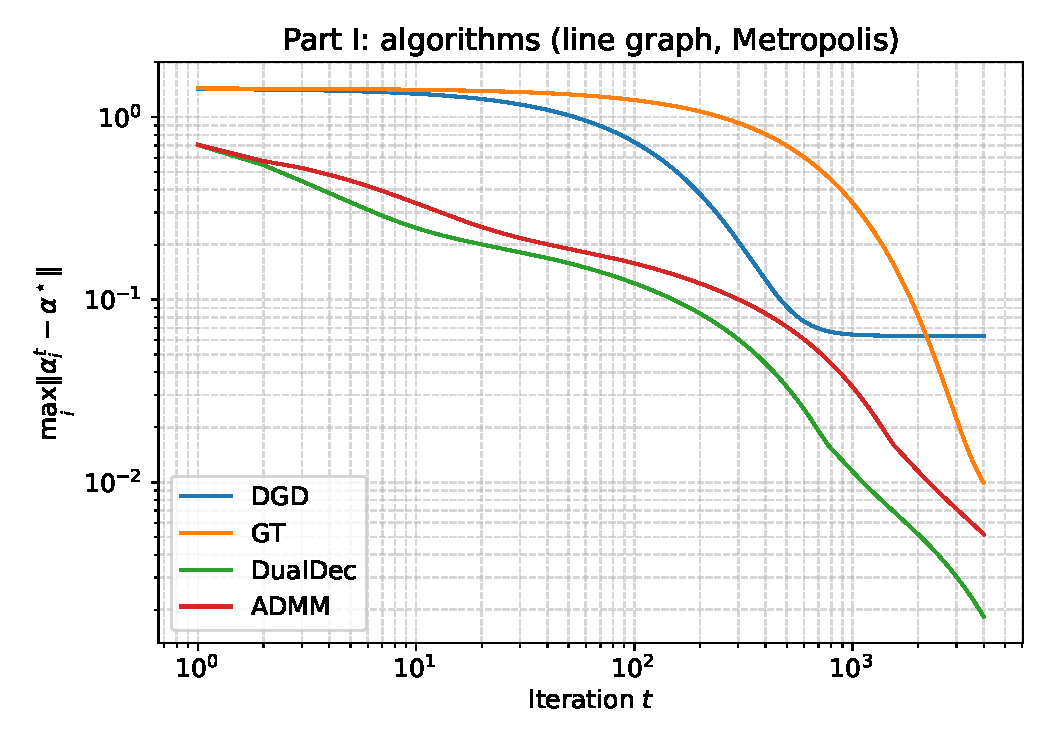
\includegraphics[width=0.85\linewidth]{figures/part1_algorithms_line.pdf}
  \caption{Optimality gap $\max_i\|\alpha_i^t-\alpha^\star\|$ vs.\ iterations (log-log).}
\end{figure}

\section{Part II: FedAvg}
FedAvg with batch size $B$, $C$ clients, $E$ local epochs. Objective gap $F(\alpha^t)-F(\alpha^\star)$ vs.\ rounds. See \texttt{part2\_fedavg\_E.pdf}. Partial participation: \texttt{part2\_fedavg\_partial.pdf} (fixed $E=5$, compare $C$); \texttt{part2\_fedavg\_partial\_E.pdf} (fixed $C=3$, compare $E\in\{1,5,50\}$).

When local shards (here $20$ points per client) are not IID, FedAvg suffers \emph{client drift}. We implement \textbf{SCAFFOLD} (Karimireddy et al., 2020): each client $i$ keeps a control variate $c_i$, the server keeps $c$, and local updates use $\nabla f_i - c_i + c$; after $K$ local steps, $c_i \leftarrow c_i - c + (x^t-y_i^K)/(\eta K)$ and $c$ is aggregated. See \texttt{part2\_scaffold.pdf}.

\section{Part III: DGD-DP}
DGD with Laplacian noise on exchanged states; noise scale tied to $\epsilon$-DP budget (course Ch.~9, arXiv:2202.01113). See \texttt{part3\_dgd\_dp.pdf}.

\section{Conclusion}
Comment on graph spectrum $\gamma$, consensus vs.\ noise, and FedAvg bias with large $E$.

\end{document}
